\section{Fixed points, stability and Hopf bifurcations} \label{Sec:fix_pnt_stab_Hopf_bif}
Recall the conditions on the parameters: they are all positive, with $\alpha+\beta<1$ and $1\neq \eta>\frac{\epsilon}{1+\epsilon}$. The following theorem that the authors postulated in the main paper \cite{antoci_poverty_2011} deals with the problem of the \underline{existence} and numerosity of stationary states (also known as \underline{fixed points}) of the dynamic system \eqref{eqn:K_dot_E_dot_L_dot}. I mention also the proof because it includes some formulas used in a second moment.
\begin{thm} \label{thm:existence_and_num_equilibria}
	System \eqref{eqn:K_dot_E_dot_L_dot} has one stationary state if $\alpha+\gamma>1$; one or zero stationary states if $\alpha+\gamma=1$; one or two stationary states if $\alpha+\gamma<1$.
\end{thm}
\begin{proof}
	A stationary state $P^*=(K^*,E^*,L^*)$ of \eqref{eqn:K_dot_E_dot_L_dot} have to satisfy the following relations 
	\begin{equation} 
		\begin{split}
			&L^* = \frac{\beta}{\beta+\epsilon}\\
			&K^* = \frac{\alpha}{\delta\theta}E^*(\bar{E}-E^*) \\
			&g(E^*):=E^*+ \delta\Big(\frac{\beta}{\beta+\epsilon}\Big)^{\frac{\beta}{1-\alpha}} \Big(\frac{\alpha}{\theta}\Big)^{\frac{\alpha}{1-\alpha}} {(E^*)}^{\frac{\alpha+\gamma-1}{1-\alpha}} =\bar{E}
		\end{split}
	\end{equation}
	or equivalently,
	\begin{equation} \label{eqn:fixed_pnt_satisfy}
		\begin{split}
			&L^* = \frac{\beta}{\beta+\epsilon}\\
			&K^* = \Big(\frac{\beta}{\beta+\epsilon}\Big)^{\frac{\beta}{1-\alpha}} \Big(\frac{\alpha}{\theta}\Big)^{\frac{1}{1-\alpha}}{(E^*)}^{\frac{\gamma}{1-\alpha}} \\
			&g(E^*):=E^*+ \delta\Big(\frac{\beta}{\beta+\epsilon}\Big)^{\frac{\beta}{1-\alpha}} \Big(\frac{\alpha}{\theta}\Big)^{\frac{\alpha}{1-\alpha}} {(E^*)}^{\frac{\alpha+\gamma-1}{1-\alpha}} =\bar{E}
		\end{split}
	\end{equation}
	Hence the graph of $g(E)$ intersects the line $E=\bar{E}$ exactly at one point if $\alpha+\gamma>1$, at most at one point if $\alpha+\gamma=1$, at zero, one or two points if $\alpha+\gamma<1$, while $K^*$ is an increasing function of $E^*$ (see Fig. \ref{fig:graph_g(E)}).  
\end{proof}

Observe that, if $\alpha+\gamma<1$, then there exists one stationary state only if the minimum of the function $g(E^*)$ coincides with the value $\bar{E}$ (assumed to be the carrying capacity of the natural resource); so, generically, the stationary states are zero or two.\\
By \eqref{eqn:fixed_pnt_satisfy}, when two stationary states exist, $P_1^* = (K_1^*,E_1^*,L^*)$ and $P_2^* = (K_2^*,E_2^*,L^*)$, then $K_1^* < K_2^*$ and $E_1^* < E_2^*$; so $P_2^*$ Pareto-dominates\footnote{The meaning of the term "Pareto-domination" is described on web at \url{https://en.wikipedia.org/wiki/Pareto_efficiency}.} 
$P_1^*$.
If the economy approaches the latter, then a \textit{tragedy of commons}\footnote{Term that refers to a situation in which individuals with access to a public resource (also called a \textit{common}) act in their own interest and, in doing so, ultimately deplete the resource. Examples are coffee consumption, over-fishing, fast fashion, groundwater use, etc. For more details take a look at \url{https://en.wikipedia.org/wiki/Tragedy_of_the_commons}.} 
scenario emerges, characterized by over-exploitation of the natural resource and by low physical capital accumulation (labor input is equal to $L^* = \frac{\beta}{\beta+\epsilon}$ at both stationary states).\footnote{It is worth to stress that, even if a trajectory approaches $P_2^*$, it does not represent an optimal growth path, since environmental externalities are not internalized by economic agents.}
\begin{figure}
	\centering
	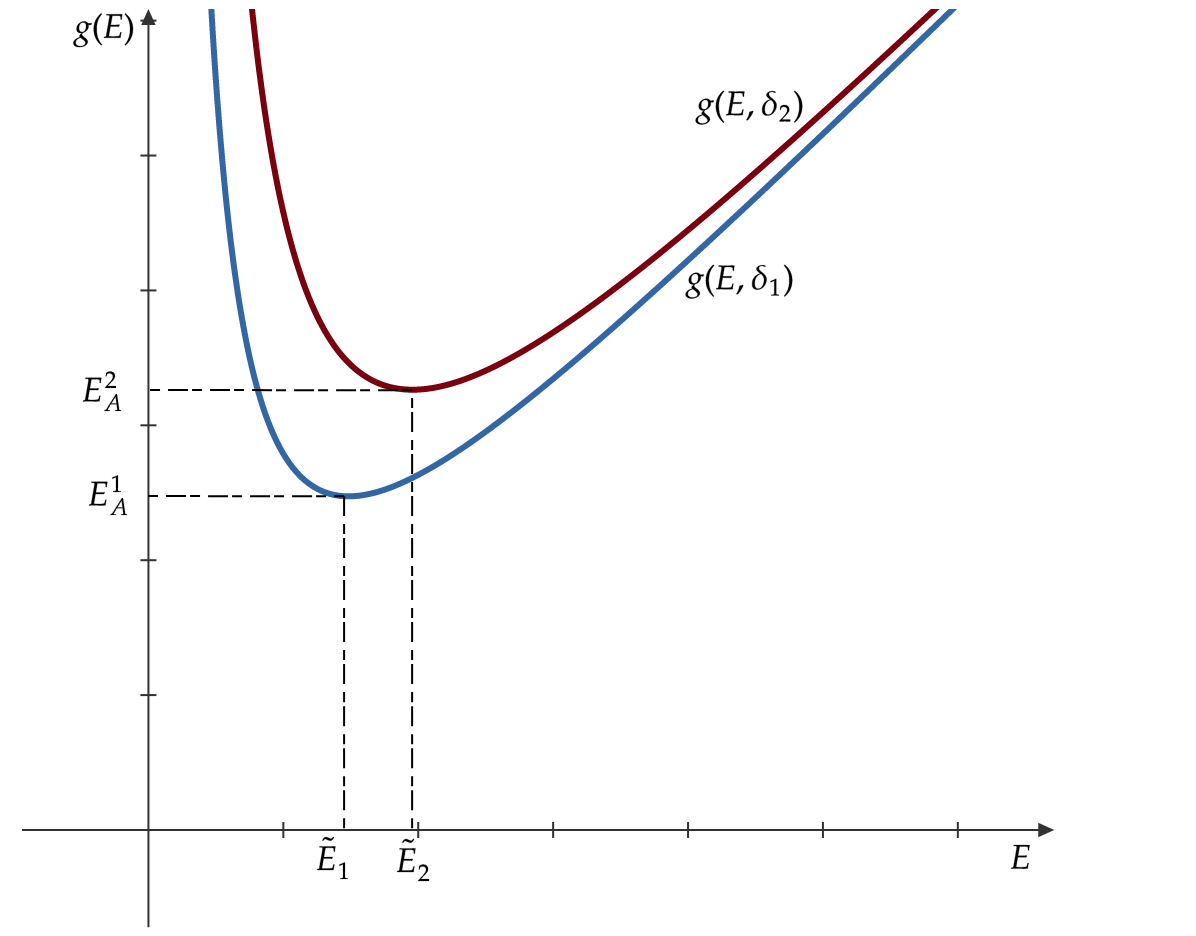
\includegraphics[width=9cm]{graph_g(E).png}
	\caption{The graph of $g(E)$, $E>0$, is drawn for values $\delta_1<\delta_2$ of $\delta$ (clearly in the case of $\alpha+\gamma<1$), when $\delta$ increases then both the coordinates of the minimum point, i.e. $(\tilde{E}, E_A)$ with $E_A=g(\tilde{E})=(\frac{2-2\alpha-\gamma}{1-\alpha-\gamma})\tilde{E}$, increase.}
	\label{fig:graph_g(E)}
\end{figure}

Now, let $P^*=(K^*,E^*,L^*)$ be a stationary state of \eqref{eqn:K_dot_E_dot_L_dot} and consider the Jacobian matrix of the same system \eqref{eqn:K_dot_E_dot_L_dot} evaluated at $P^*$
$$
Jac(P^*)=J^* =
\begin{bmatrix}
	0 & 
	0 & 
	\frac{\partial\dot{K}}{\partial L} \\[1ex] % <-- 1ex more space between rows of matrix
	\frac{\partial\dot{E}}{\partial K} & 
	\frac{\partial\dot{E}}{\partial E} & 
	\frac{\partial\dot{E}}{\partial L} \\[1ex]
	\frac{\partial\dot{L}}{\partial K} & 
	\frac{\partial\dot{L}}{\partial E} & 
	\frac{\partial\dot{L}}{\partial L}
\end{bmatrix}
$$
where, by straightforward computations
\begin{equation} \label{eqn:part_deriv_Kdot_Ldot_Edot}
	\begin{split}
		\frac{\partial\dot{K}}{\partial L} &= \frac{\beta+\epsilon}{\delta\beta}E^*(\bar{E}-E^*)\\
		\frac{\partial\dot{E}}{\partial K} &=-\delta\theta \\
		\frac{\partial\dot{E}}{\partial E} &=\bar{E}(1-\gamma)-E^*(2-\gamma)\\
		\frac{\partial\dot{E}}{\partial L} &=-(\beta+\epsilon)E^*(\bar{E}-E^*)\\
		\frac{\partial\dot{L}}{\partial K} &=\frac{f(L^*)}{f'(L^*)}\frac{\delta\theta}{E^*} \Bigg[\frac{\theta(1-\alpha)}{\alpha\eta(\bar{E}-E^*)}-\gamma\Bigg]\\
		\frac{\partial\dot{L}}{\partial E} &=\frac{f(L^*)}{f'(L^*)}\frac{\gamma}{E^*} \Bigg[ (1-\gamma)(\bar{E}-E^*)-E^*-\frac{\theta}{\eta} \Bigg]\\
		\frac{\partial\dot{L}}{\partial L} &=\frac{f(L^*)}{f'(L^*)}(\beta+\epsilon) \Bigg[ \frac{\theta(\beta+\epsilon)}{\epsilon}-\frac{\theta}{\eta}-\gamma(\bar{E}-E^*) \Bigg].
	\end{split}
\end{equation}
Another important theorem from the paper holds: 
\begin{thm} \label{thm:num_eigenval_from_Jac}
	If the stationary state is unique with $\alpha+\gamma\geq1$, or, in case of two stationary states, is the one with the larger $E^*$, then $J^*$ has an odd number of positive eigenvalues; instead, if, in case of two stationary states, $P^*$ corresponds to the one with the smaller $E^*$, then $J^*$ has an odd number of negative eigenvalues.
\end{thm}
\begin{proof}
	By computing $det(J^*)$, one can check that
	\begin{equation} \label{eqn:sign_det_J*}
		sign[det(J^*)] = sign[(2-2\alpha-\gamma)E^*-(1-\alpha-\gamma)\bar{E}]
	\end{equation}
	It follows that, when the stationary state is unique and $\alpha+\gamma\geq1$, then $det(J^*) > 0$. Vice versa, when two stationary states exist, implying $\alpha+\gamma<1$, then it follows from \eqref{eqn:sign_det_J*}, by observing Fig. \ref{fig:graph_g(E)}, that $det(J^*)$ has the same sign of $g'(E^*)$, which proves the theorem. 
\end{proof}

Considering a non-generic case when a unique stationary state exists under the condition $\alpha+\gamma<1$, then $det(J^*)=0$ holds and the stationary state is not hyperbolic (in fact, a saddle-node bifurcation occurs). Consequently, if one looks for an attracting stationary state, that one have to restrict his/her analysis to the case when, under the assumption $\alpha+\gamma<1$, two stationary state exist, $P_1^*$ and $P_2^*$, with $E_1^* < E_2^*$ and $K_1^* < K_2^*$. Here the scientist aim to show that, in such a context, $P_1^*$ can be attracting for suitable values of the parameters. Along the trajectories belonging to the basin of attraction of $P_1^*$ the over-exploitation of the natural resource drives the economy towards a \textit{tragedy of commons} scenario.

First of all, if $\alpha+\gamma<1$, a necessary and sufficient condition for the existence of two stationary states is
\begin{equation}
	\bar{E}>E_A := g(\tilde{E})=\Bigg(\frac{2-2\alpha-\gamma}{1-\alpha-\gamma}\Bigg) \tilde{E}
\end{equation}
where $\tilde{E}$ is the only positive value satisfying $g'(\tilde{E})=0$. \\
Straightforward computations yield 
\begin{equation}
	E_A =(2-2\alpha-\gamma)\Bigg[\frac{\delta^{1-\alpha}}{(1-\alpha)^{1-\alpha}(1-\alpha-\gamma)^{1-\alpha-\gamma}} \Bigg(\frac{\beta}{\beta+\epsilon}\Bigg)^{\beta} \Bigg(\frac{\alpha}{\theta}\Bigg)^{\alpha}\ \Bigg]^{\frac{1}{2-2\alpha-\gamma}}
\end{equation}
Thus, $E_1^*<\tilde{E}<(\frac{1-\alpha-\gamma}{2-2\alpha-\gamma})\bar{E}$.
\underline{From now the index 1 will be omitted}. 

The well-known Routh–Hurwitz Criterion (see Hurwitz \cite{hurwitz_conditions_1964}) yields that $J^*$, the Jacobian matrix at $P^*$, has three eigenvalues with negative real part if and only if
\begin{equation} \label{eqn:det_J*_neg}
	det(J^*)<0,
\end{equation}
\begin{equation} \label{eqn:cond_sigma_rho_stab}
	\begin{split}
		\sigma(J^*) &= \frac{\partial\dot{E}}{\partial E}\frac{\partial\dot{L}}{\partial L}-\frac{\partial\dot{E}}{\partial L}\frac{\partial\dot{L}}{\partial E}-\frac{\partial\dot{K}}{\partial L}\frac{\partial\dot{L}}{\partial K}>0\\
		\rho(J^*) &= -\sigma(J^*)\cdot trace(J^*)+det(J^*)>0
	\end{split}
\end{equation}
The last inequality, in particular, guarantees the non-existence of complex eigenvalues with non-negative real part. In fact, when $\rho(J^*)$ crosses the origin value $0$, the real part of two complex conjugate eigenvalues changes sign, causing, generically, a Hopf bifurcation.
Remember that the condition \eqref{eqn:det_J*_neg} is always verified at $P^*$ (see \eqref{eqn:sign_det_J*}). As for the condition \eqref{eqn:cond_sigma_rho_stab}, the authors of the paper stated the following lemma.
\begin{lemma}
	If 
	\begin{equation} \label{eqn:lemma_3}
		\eta\geq \frac{\epsilon}{\epsilon+\alpha\beta} \quad \text{and} \quad \bar{E}>E_B=\frac{\theta(\beta+\epsilon)(2-2\alpha-\gamma)}{\alpha\beta\gamma\eta}
	\end{equation}
	then the condition $\sigma(J^*)>0$ is verified.
\end{lemma}
\begin{proof}
	By recalling \eqref{eqn:part_deriv_Kdot_Ldot_Edot}, straightforward computations lead to 
	$$ sign[\sigma(J^*)] = sign\Bigg[\Bigg(\frac{\beta+\epsilon}{\epsilon}-\frac{1}{\eta}\Bigg)(\bar{E}-2E^*)-\frac{\theta(1-\alpha)(\beta+\epsilon)}{\alpha\epsilon\eta}\Bigg] $$
	So, since $E^*<(\frac{1-\alpha-\gamma}{2-2\alpha-\gamma})\bar{E}$, the assumptions of the lemma imply $\sigma(J^*)>0$.
\end{proof}
One shall now compute $trace(J^*)$; observing that $\frac{f(L^*)}{f'(L^*)}=\frac{\beta\epsilon\eta}{(\beta+\epsilon)[\eta(\beta+\epsilon)-\beta\epsilon]}$, one obtain $$trace(J^*)=a(\bar{E}-E^*)-E^*+b$$ where 

\begin{equation}
	a:=\frac{\eta[(1-\gamma)(\beta+\epsilon)-\beta\gamma\epsilon]-\beta\epsilon(1-\gamma)}{\eta(\beta+\epsilon)-\beta\epsilon}, \qquad b:=\frac{\beta\theta[\eta(\beta+\epsilon)-\epsilon]}{\eta(\beta+\epsilon)-\beta\epsilon}.
\end{equation}
Then the results of the so far done analysis, aimed at detecting an attracting stationary state(or fixed point), are summarized by the following theorem.
\begin{thm} \label{thm:result_of_analysis}
	Let $\alpha+\gamma<1$ and $\bar{E}>E_A$, so that system \eqref{eqn:K_dot_E_dot_L_dot} has two stationary states, $P_1^*$ and $P_2^*$, with $E_1^*<E_2^*$ and $K_1^*<K_2^*$. Then there exist values of the parameters for which $P_1^*$ is a sink, while $P_2^*$ is a saddle with a two-dimensional stable manifold. Moreover, in such a case, take $\bar{E}$ as a bifurcation parameter. As $\bar{E}$ is increased, $P_2^*$ does not change its nature (i.e. it remains a saddle with a two-dimensional stable manifold), whereas $P_1^*$ can undergo one, two or no Hopf bifurcations.
\end{thm}
\begin{proof}
	Omitted. See Appendix A of the usual paper \cite{antoci_poverty_2011}.
\end{proof}
Notice that the sufficient conditions for local indeterminacy given above depend on the intertemporal elasticity of substitution\footnote{In economics, intertemporal elasticity of substitution, IES, is a measure of responsiveness of the growth rate of consumption to the real interest rate. For more details see \url{https://en.wikipedia.org/wiki/Elasticity_of_intertemporal_substitution}.} 
and can be satisfied both in case $\eta<1$ (i.e. elasticity of substitution greater than 1) and in case $\eta>1$ (i.e. elasticity of substitution lower than 1): in fact, previously they have assumed $\eta\geq \frac{\epsilon}{\epsilon+\alpha\beta}$. Furthermore, those conditions require that the impact of the production process of output (measured by $\delta$) is high enough and/or the subjective discount rate $\theta$ is low enough. Finally, the elasticity $\gamma$ of the production function with respect to the natural capital $E$ must be not too high, that is $\alpha+\gamma<1$, while social returns to scale can be constant or decreasing, that is $\alpha+\beta+\gamma\leq1$.


